\documentclass[11pt]{article}
\usepackage{evolution}
\usepackage{bibentry}
\setstretch{1}
\parindent 0pt
\parskip 8pt

\renewenvironment{quote}{\bigskip\noindent\itshape\ignorespaces}{\smallskip}

\begin{document}

\hfill \today

Dear Dr. Schoen and reviewers,

\medskip
Thank you very much for your close reading of our manuscript and supportive comments. We appreciate your constructive suggestions, each of which we address below. You will find a big difference on the number of  models  that we have fitted for the revision based on your suggestions (originally 12 now 29). The two main reasons to increase the number of models were to first address one key question by made by all referees about the symmetry of the hidden states, and second to address a remaining question about adding complexity to two-state models. For the symmetry of the hidden states  question we found that is relevant to have asymmetric hidden state rates and in our case, it strengthened the differences amongst net diversification rates. The second question,  comes from a vague idea that we had while submitting the first version of this article: by increasing from two to three states the models, are we explaining better the history of diversification? This second question could not be addressed directly by model comparison statistics because the two-state and three-state models need different input (i.e. (0,1) versus (0,1,2)). However, the species and the tree are the same and our intuition indicated that they should carry the same biological evidence despite any particular coding needed as input. During this revision, we figured a way to recode the three-state models to make them equivalent to the two-state models (the new lumped models). Thanks to this equivalency, two-state and three-state models can now be compared to argue for the importance of adding key trait information and states in diversification analyses. We also revised the original dataset thanks to the suggestion of Reviewer 1, and we were able to correct discrepancies with previous dataset as well as add more sample (651 taxa).

We hope the changes and the new models are satisfactory and exciting to you and the reviewers.

\medskip
Sincerely,

Rosana Zenil-Ferguson, on behalf of all authors
% E: Pardon my speaking for you, Rosana. :)  Obviously change whatever wording below---starting to draft responses just helped me think through the requests.
% R: I'm super excited now as you can see


%--------------------------------------------------
\section{Editor}
%--------------------------------------------------
\vspace{-11pt}

\begin{quote}
Thanks for submitting your work to New Phytologist.
We have back the referee comments now, and in general all three referees found the work to be novel and interesting.
Congratulations on accomplishing such a nice study.

Of course, the referees also had a number of critical comments and suggestions for improving the manuscript and so I am suggesting that your paper be accepted with `major revision' due to the number and nature of the comments, some of which I agree with, and others perhaps not.
I will be interested to hear your reasoning for either accepting or not accepting these suggestions when you re-submit the revised manuscript.

Perhaps foremost among the issues that should be addressed in the revision is that the referees felt that readers are not likely to be familiar with the SSE-type models that incorporate hidden states.
More background information should be provided to make it clearer how the incorporation of hidden states alters the approach and especially the interpretation of results.
This becomes especially important for understanding the multistate models, and for later on, for following your reasoning and justification in reducing the number of parameter states in said models.
Related to the issue of providing useful background information, Referee \#2 suggests that readers who are less familiar with mating system function will benefit by having a clearer exposition of the causal links between polyploidization and the breakdown of SI, something else I too think would help the paper.

Both Referees \#2 and \#3 highlight the issue of symmetry in transition rates, and from what little I know about parameter estimation in these types of models, I am partial to the suggestion of this referee that such a constraint could influence the estimation of diversification rates.

Please also go though the other referee comments which when acted upon should improve the readability of the paper.

Best wishes,

Dan Schoen
\end{quote}

Thank you for assembling these substantive reviews.
We have provided more background information on interpreting the hidden state models, and on the relationship between polyploidization and breakdown of GSI.
These and other changes are detailed below.

%--------------------------------------------------
\section{Referee 1}
%--------------------------------------------------
\vspace{-11pt}

\begin{quote}
I think this is an excellent paper, both in its analytical approach, and in its biological insights.
In particular, I think the general approach---gradually adding complexity to the models, and comparing their inferences with those from simpler models and the literature---is very effective.
In addition, the use of hidden state and multistate SSE models provides a useful framework for other macroevolutionary studies. 
Most of my comments are specific things (grammar, etc.), although I think the paper would benefit from a slightly pulled-back concluding bit---what from these results do the authors think is broadly applicable, and what is likely specific to Solanaceae and S-locus incompatibility systems?
\end{quote}

Thank you for the kind words.
We have substantially revised the Discussion, including providing more perspective on the general versus specific findings. % TODO

\begin{quote}
Could the last two sentences of the abstract be made more concrete?
The phrases ``generates interesting outcomes'' and ``affects conclusions about \ldots different evolutionary pathways'' are both pretty vague (the authors do an impressive job of summarizing complex ideas in this abstract, and maybe it's as specific as possible given word number constraints etc).
\end{quote}

We improved this wording.

\begin{quote}
The introduction is broad, and generally well supported, but a little disjointed, and additional literature on the macroevolutionary consequences of each of polyploidy and breeding system could be included.
As well as their correlation with each other---this is a well-acknowledged problem.
Ln65 says this nicely, but this point could be introduced (with the appropriate literature cited) earlier.
Also, the introduction is explicitly limited to angiosperms, which doesn't seem necessary---other landplant lineages (and non-plants, for that matter) also have ploidy and breeding system variation.
\end{quote}

okay % TODO

\begin{quote}
--35 Is the Soltis et al.\ 2014 citation appropriate here?
That paper doesn't present much by way of new data
\end{quote}

check % TODO

\begin{quote}
--55 change ``effect disruption'' to ``disrupt''
\end{quote}

Fixed.

\begin{quote}
--57 vague pronoun -- ``this'' (as a general rule, don't use ``this'', ``that'' etc by themselves -- follow them with the noun that they're referring to)

--use commas before ``which''; if no comma, use ``that''
\end{quote}

We reworded this whole paragraph, as part of better explaining how polyploidization disables gametophytic SI.

\begin{quote}
--83 Nitpicky, but is it accurate to refer to this as a false-positive problem?
``False positive'' implies to me the erroneous rejection of the null, but in this case the situation is more of the null being mis-specified with respect to the question the researcher is after.
The null---no rate variation---is correctly rejected.
This section probably should include a reference to Rabosky and Goldberg.
\end{quote}

We reworded this whole paragraph, as part of better explaining the SSE family of models.

\begin{quote}
--115 I'm uncomfortable with this way of handling multiple cytotypes.
The most commonly reported cytotype could easily not be the most common cytotype in the wild (I assume that most taxa are represented by relatively few counts), and regardless, there is biology here.
Specifically, this methodology would artificially reduce the number of ploidy changes (if a taxon is polymorphic for ploidy, there's at least one event there), and the omitted changes would be disproportionately those towards the tips of the phylogeny, so not only would rates be depressed, but the bias is of a sort that the estimation of diversification parameters is particularly sensitive to (the authors will understand why this is so).
\end{quote}
We acknowledge this is a potential problem. It is true that chromosome number multiplicity can bias coding towards more (or less) transitions when it heavily depends on the most common cytotype. For the majority of species (~85\%)  the ploidy was not directly dictated by us but by the original sources of the data. In the originally sources ploidy has been classified not only most common cytotype but geographical distribution, multivalence, and/or  genome sizes. The remaining 15\% of the sample is what we assigned based on genus or family cytotype multiplicity. We cross-validated all of the assignments with the data from \citet{robertson_2011} where ploidy was assigned via a chromosome number change model using ChromEvol \citep{mayrose_2010}. We differ in exactly 35 species from \citet{robertson_2011} were we found a new reference or a new chromosome count. Classifying using a chromosome number change models only could also suffer from inflation of polyploidy events due to the lack of diploidization parameters, we found some specific species in the  \citet{robertson_2011} sample that were clearly aneuploids (one chromosome difference) that were classified as polyploids using chromosome number models, we manually corrected for those hoping to minimize obvious mistakes.

\begin{quote}
--130 I don't follow this discussion.
There's a self-incompatible pentaploid?
How is it even sexual?
Regardless, the discussion of this pentaploid should be more clearly integrated back into the central argument here, about the absense of SI polyploids (I think that's the central argument?).
\end{quote}

%B: I edited the manuscript (methods.tex) as explained below:
We removed the discussion and simply reference a more detailed treatment of this single individual.
We agree that this observation by \citet{camadro_1981} may be distracting, and now instead  point the reader to our previously published paper \citep{robertson_2011}, where the possible existence of pentaploid that fails to set seed following self-pollination is discussed at some length.

%Although SI populations frequently contain some SC individuals, and diploid populations frequently contain some polyploid individuals, in no case did we find convincing data for a naturally occurring SI polyploid population  \citep[discussed in][]{robertson_2011}.
%B rm: The single instance of an SI polyploid individual appears to be an allopentaploid hybrid of \textit{Solanum oplocense} Hawkes x \textit{Solanum gourlayii} Hawkes, reported by \citet{camadro_1981}.
% Under exceedingly rare circumstances, it is possible for polyploids containing multiple copies of S-loci to remain SI, so long as they express a single allele at the S-locus \citep[discussed in][]{robertson_2011}.

\begin{quote}
--133 change ``SI and polyploidy populations'' to ``polyploid SI populations'' (there are lots of polyploid populations, and lots of SI ones, too)
\end{quote}

Fixed.

\begin{quote}
--140 I lost track a little of how the data were coded -- maybe add an explicit statement as to how many tips had both forms of data, how many had only breeding system info, how many had only ploidy info (I see now, after the fact, that those data are included in the figure), and how missing data were handled
\end{quote}

Fixed.

\begin{quote}
--It's not intuitive to me what the effects of forcing the hidden state change rates to be symmetrical are.
Did the authors investigate this?
Or has it been explored in the literature?
Similarly, it seems to me that fixing the transition rates of the observed characters to be independent of the hidden state could do weird things---the point of these SSE models is that state change rates and state-dependent diversification rates need to be co-estimated
\end{quote}

We appreciate this suggestion and we followed it. The main result after fitting models with symmetric vs. asymmetric rates is that the direction  of the results does not change but the amount of difference amongst net diversification posterior distributions does. We found using Bayes factors that a model including asymmetric hidden rates is preferred over a model with equal hidden rates. Also,  the asymmetry in the trait rates have moderate to not support of being better than a model with equal trait transition rates.  %TODO put number.

\begin{quote}
--221  Propagation
\end{quote}

Fixed.

\begin{quote}
--I would be more comfortable if each model was run at least twice, independently, to better assess whether the MCMC has indeed converged
\end{quote}
Unfortunately, we weren't able to run multiple chains for all models due to some limitations to our computer resources. However, we were able to test for the convergence of  three key models using Gelman's $\hat{R}$ test statistic. We tested convergence with two runs of 130,000 generations (after 5,000 generations of burn-in) for models D/P (BiSSE), D/P+A/B asym (HiSSE) and ID/CD/CP+A/B asym (MuHiSSE). The statistics as well as the Gelman plots in  \ref{figure:convergencestats} show that with that number of generations the models were converging. We increased the number of generations to be safe for all the models that we did not test and visually assessed the mixing of  models on top of demanding ESS larger than 200 for parameters. 

\begin{figure}
    \centering 
      \begin{minipage}[b]{0.33\textwidth}
    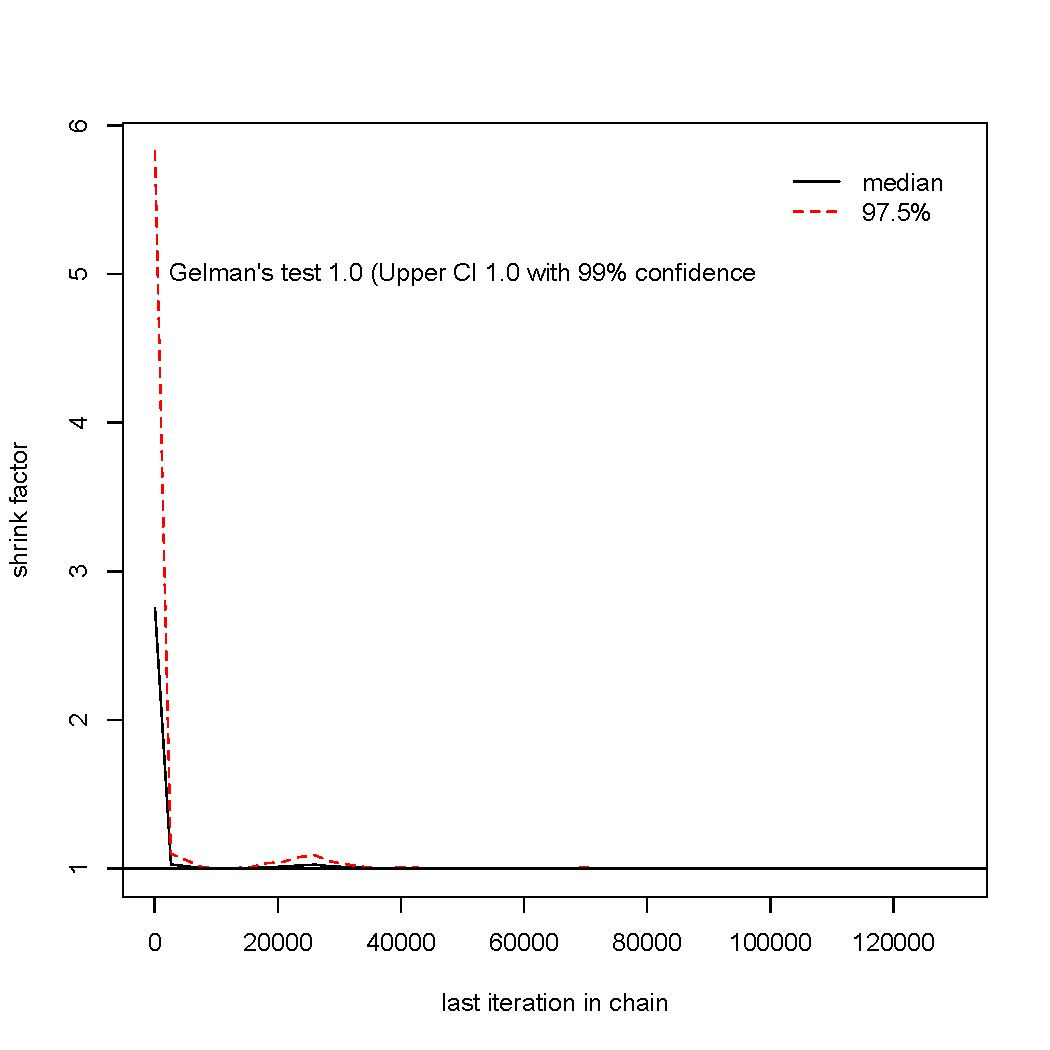
\includegraphics[width=\textwidth]{Gelmanbissenodip.pdf} 
    \end{minipage}
    \begin{minipage}[b]{0.33\textwidth}
        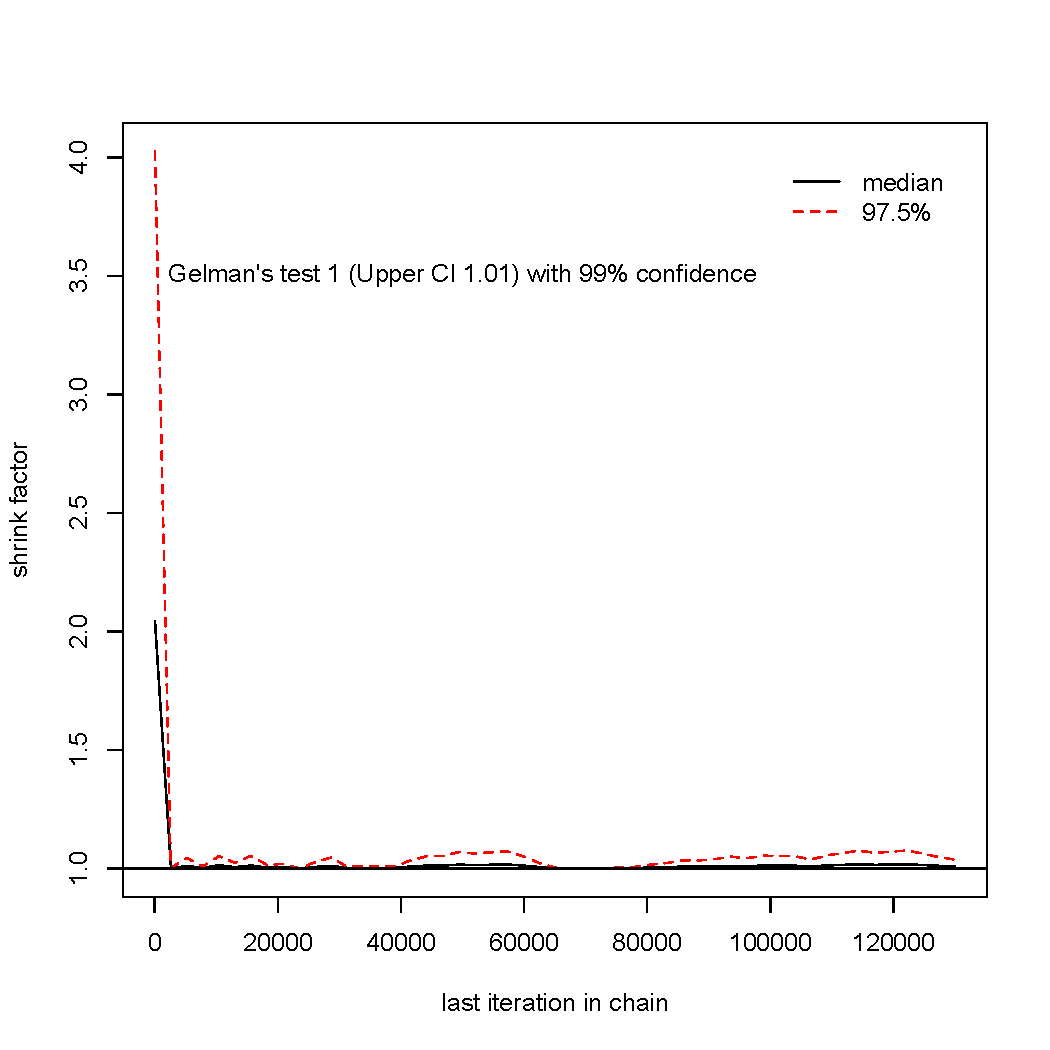
\includegraphics[width=\textwidth]{Gelmanhissenodipasym.pdf}
        \end{minipage}
    \begin{minipage}[b]{0.33\textwidth}
             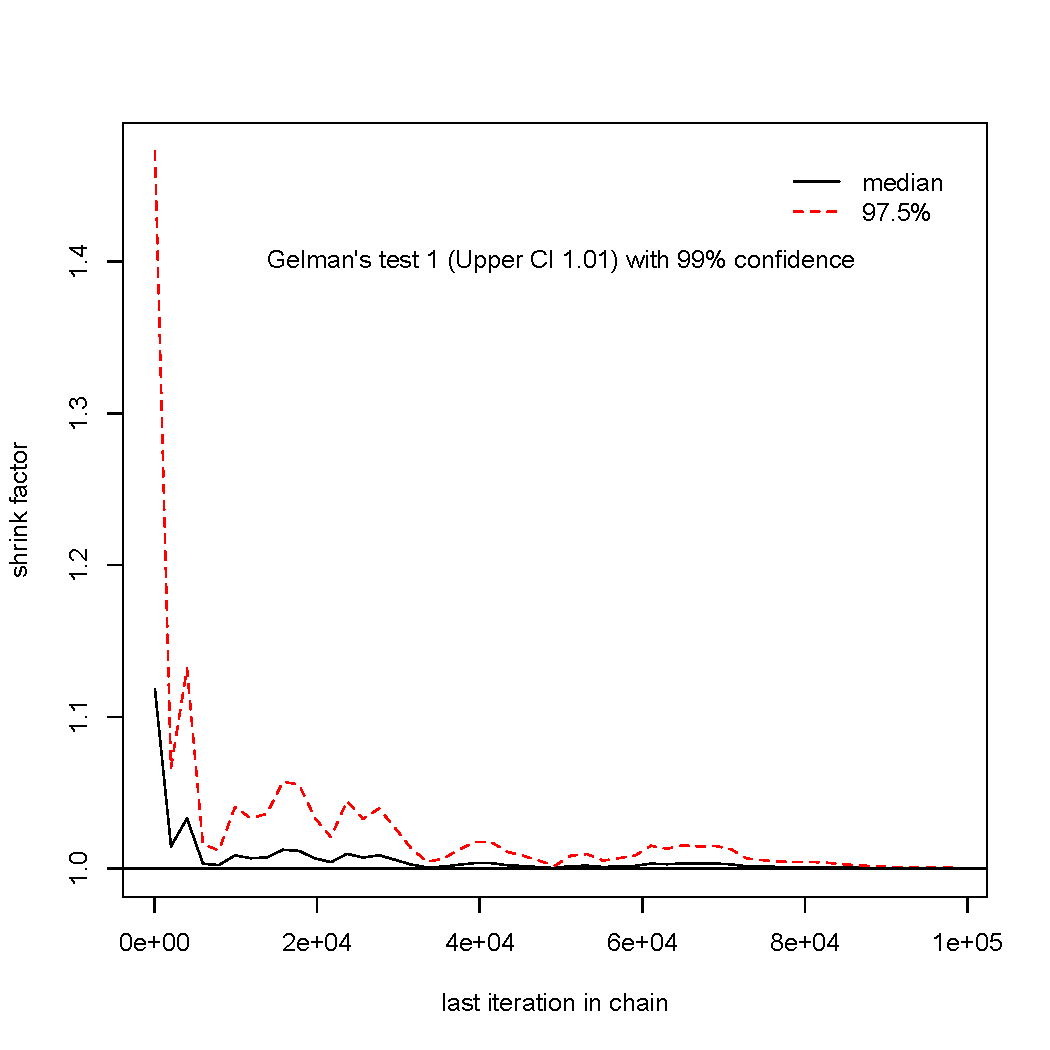
\includegraphics[width=\textwidth]{Gelmanmuhissenodipasym.pdf}
                 \end{minipage}
    \caption{ Convergence statistics and Gelman plots for D/P (BiSSE), D/P+A/B asym (HiSSE) at the top and ID/CD/CP+A/B asym (MuHiSSE,bottom). Upper limits of Gelman's test statistics should be close to 1 for an MCMC to be considered convergent.}
    \label{figure:convergencestats}
\end{figure}


\begin{quote}
--the use of run time as a description of the analysis seems odd to me.
As a reader, I'm not interested in the power of a given computer -- I want to know how many generations the MCMC was run for, what the ESSs are, etc.
\end{quote}
We ran each model for 200,000 generations. Unfortunately, we don't have access to more of 96 hours of computational time to increase those but we have calculated the convergence as indicated above.

\begin{quote}
-325  These analyses (by accounting for diversification) may take care of this issue, but is there a problem with these results being driven by a non-stationary process being modeled as a stationary one?
\end{quote}

This was a point worth considering, but our model does not assume stationarity.
In Fig.~4, the contributions of each pathway are functions of time.
We can see there both the short-term and long-term behavior.
% Rosana, what do you think?- I think this is a good answer- I think it is good

\begin{quote}
--340  Sentence fragment
\end{quote}

Fixed. % TODO

\begin{quote}
--beginning of the Discussion is perhaps unnecessary -- it's more like Introduction material
\end{quote}

consider % TODO

\begin{quote}
--are the results from the analyses that include diploidization coherent?
I'm not sure how to phrase this -- I guess I'm asking if there's any suggestion that that parameterization is indeed capturing the biological phenomenon of diploidization, or is it just soaking up noise?
\end{quote}

The soaking noise comes from the hidden state so in the presence of hidden states finding that diploidization matters is key. All the Bayes factors indicated strong support for models that include diploidization. However, the diploidzation parameter per se is difficult to estimate (wide credible intervals) mainly because diploidization is a genome size process that can be partially or minimally recover from ploidy data. This is the reason why we do not overstate this finding,  the importance of diploidization needs to be studied using genomes.

\begin{quote}
--I think this is an excellent point -- ``SI, which is itself associated with a faster diversification rate, is the breeding system context in which many diploids occur.''
Perhaps an discussion of the extent to which these results are extendable to other plant groups would be appropriate, versus what is likely to be specific to this system
\end{quote}

Seems reasonable. % TODO

\begin{quote}
--366  I would use a more compelling descriptor than ``interesting'' to describe these traits
\end{quote}

Fixed.

\begin{quote}
--390  I don't fully follow.
Could this comparison be expanded upon?
And maybe avoid the parameter notation, and just describe the rates being compared.
\end{quote}

consider % TODO

\begin{quote}
--400  Didn't Mayrose et al.\ 2011 and Magnuson-Ford \& Otto 2012 look at this (cladogenic change)?
\end{quote}

Yes. We adjusted the text accordingly.

\begin{quote}
--408  In what way are the present results in conflict with other reports from the literature?
(It's not clear, at least at first, where this conflict lies)
\end{quote}

consider % TODO

\begin{quote}
--410  ``as self-incompatibility loci''?
\end{quote}

Fixed.

\begin{quote}
--417  Why would the rates for diploids be inflated?
So the diploids were ancestrally polyploidy -- why would that alter the rate inferences?
\end{quote}

consider % TODO

\begin{quote}
--430  remove the comma
\end{quote}

Fixed.

\begin{quote}
--436  use ndashes to indicate ranges (rather than hyphens)
\end{quote}

Fixed.

\begin{quote}
--437-8 I don't understand this sentence
\end{quote}

Fixed.

\begin{quote}
--455  I don't quite follow where this section is leading -- I think these loose ends should be explicitly tied together.
There are reports of paleopolyploidy in Solanaceae and relatives, but there are reasons to be skeptical of them?
\end{quote}

consider % TODO

\begin{quote}
--457  differ by six..
\end{quote}

Fixed.

\begin{quote}
--467  focal trait
\end{quote}

Fixed.

%--------------------------------------------------
\section{Referee 2}
%--------------------------------------------------
\vspace{-11pt}

\begin{quote}
I really enjoyed reading the manuscript.
The subject is pertinent and interesting and the methodological approaches used are amongst the best available to answer such questions.
Polyploidy is well known to be evolutionarily correlated with self-incompatibility breakdown and their respective impact on diversification rates are best studied simultaneously.
The results presented show exactly this, but in addition show that some unknown hidden states could also affect diversification rates, suggesting that results must be interpreted with care.
These are very interesting results.
\end{quote}

We're pleased you found the results interesting!

\begin{quote}
I have two ``major'' comments.
The first is relatively easy to fix and is linked to the writing/structure of the paper.
I often had the impression that too much knowledge is assumed from the reader throughout the manuscript.
For instance, more information should be given in the intro regarding why self-incompatibility breakdowns with polyploidy (it is briefly explained, but only later in the manuscript).
Moreover, some methodological approaches could be better explained.
In particular, HISSE models are relatively recent and many readers may not know them well.
I thus think that it would be important to describe them better and also better explain the results (using biological terms) obtained.
I mention some examples below in the detailed notes where I think explanations could be added.
\end{quote}

We have rewritten parts of the manuscript, especially in the Introduction, to try to explain better the relationship between polyploidy and self-incompatibility, and the interpretations of hidden state models.
% E: I labeled the two paragraphs that I modified heavily.

\begin{quote}
My second comment has to do with the parameterization of the models.
Overall, I think that the authors have done a great job in justifying their models and explaining them.
I think it is important to mention.
In addition, their implementation of the models in revBayes is noteworthy and although not stated precisely in the manuscript, I believe this represents a great scientific contribution. 
Nevertheless, I question the decision to restrict the transition rates to and from the hidden states to be all equal.
Indeed, we have no idea that could make us think that this would be the case.
The authors justify this by ``Because our goal was to look for diversification rate differences associated with ploidy and breeding system rather than the specific effects of the hidden states, we fit a simplified version with 16 parameters.''
I am not completely convinced by this argument.
First, constraining transition rates can have an impact on the estimation of diversification rates.
Second, specifically because the authors are not interested in estimating the rates themselves, they should not be too worried about increasing the number of parameters.
This is especially true in a Bayesian framework where it is sometimes better to have overparameterized models than under-parameterized models (see Lemmon and Moriarty. 2004. Systematic Biology 53:265–277).
I think it would have been important to at least present the results of an unconstrained model to show that this decision to constrain the rates do not affect the conclusions.
\end{quote}
We have now fitted models with asymmetric hidden rates and asymmetric trait rates. We found that the former are important and strengthened the differences. We found no evidence that having all asymmetric rates is preferable over just asymmetric hidden for our specific example. %TODO (Figs and table)

\begin{quote}
Finally, I have a suggestion for the authors.
One thing that I would have like to see is a discussion regarding the distribution of the hidden states at the tip of the tree (e.g., Fig S6, S8).
The two peaks distributions obtained for the hidden and non-hidden states made me wonder if the high and low rate peaks could be restricted to specific clades on the phylogeny.
After inspecting the supplementary material, I see that it is not the case; hidden states are rather spread throughout the phylogeny.
I think this is interesting and that it could make an interesting discussion.
\end{quote}

Thanks for this suggestion, which we have incorporated in the Discussion. % TODO

% Minor points:

\begin{quote}
Line 60: Did the author mean in all polyploid examined to date?
\end{quote}

We reworded this whole paragraph, as part of better explaining how polyploidization disables gametophytic SI.

\begin{quote}
Line 70: Sentence not clear. Should explain better the results of Robertson.
\end{quote}

Fixed.

\begin{quote}
Line 87: Specify other sources. Cryptic
\end{quote}

Reworded.

\begin{quote}
Line 88: To which traits the ``these traits'' refer to?
\end{quote}

Fixed.

\begin{quote}
Line 133: Replace ``and polyploid populations'' by ``in polyploid populations''?
\end{quote}

Fixed.

\begin{quote}
Line 133-135: Should probably move this information in the intro.
\end{quote}

We now explain the effect of polyploidization on self-incompatibility more thoroughly in the Introduction.

\begin{quote}
Line 152: It would be useful to refer to the figures that illustrate the models in the methods.
It would help to understand them.
\end{quote}

Fixed. % Done: Emma did the new figure

\begin{quote}
Line 360: ``Simultaneous consideration of breeding system'' and what?
Polyploidy, hidden state?
The sentence is not clear
\end{quote}

Fixed.

\begin{quote}
Line 363: ``These results indicate that some of the effects of a hidden trait can be explained by each of the two traits under consideration''.
Not sure I understand this sentence. Is it possible to clarify?
\end{quote}

Reworded.

\begin{quote}
Line 380: The authors should explain in more details the link between the breakdown of SI and the evolution of gender dimorphism.
\end{quote}

We added a brief explanation.

\begin{quote}
Line 392: Remove one ``explained''.
\end{quote}

Fixed.

\begin{quote}
Line 392: ``our findings suggest that the effect of ploidy''.
Add ``on diversification rates'' after these words?
\end{quote}

Fixed.

\begin{quote}
Line 416: ``Unduly ignoring secondary diploidization would necessarily underestimate the rate of transitions from polyploids to diploids.''
Actually, if I understand well, models without diploidization simply fix this rate of transition from polyploidy to diploids at 0.
Am I right?
\end{quote}

consider % TODO

%--------------------------------------------------
\section{Referee 3}
%--------------------------------------------------
\vspace{-11pt}

\begin{quote}
Zenil-Ferguson et al.\ apply sophisticated modeling techniques to test for the combined impact that breeding system and ploidy have on diversification rates within Solanaceae.
These models used here include ``hidden'' states to account for the many additional unobserved trait that also impacts diversification elsewhere in the tree.
The authors find a strong correlation between ploidy and breeding system and that certain character combinations have an impact diversification.
Specifically, the authors find that as long as a lineage is diploid, being either self-compatible or incompatible result in higher diversification rates than if these breeding systems were associated with polyploids.
The main finding of diploids generally having higher diversification rates than polyploids (including a slight negative diversification rate for polyploids) is consistent with previous studies that have explored patterns of diversification in relation to ploidy in other lineages of angiosperms.
Overall, this is a very nice study, the manuscript very well written, and the results are interesting.
There is no question that this work will be of great interest to the readership at New Phytologist.

I have a few comments that I hope the authors will find useful.
\end{quote}

Thank you for this positive summary.

\begin{quote}
The first relates to the use of the hidden states in the models.
I agree completely with the rationale and meaning of including hidden states.
However, through my reading of the manuscript, I interpret the authors as using them simply to account for variation within a particular character state combination.
In other words, the authors are working under an assumption of trait-dependent diversification, with the hidden states simply providing a more nuanced view of the process.
But the authors are not considering a completely alternative view, which is that none of these trait combinations are strong drivers of diversification and that the shifts being inferred are simply coincidental.
Such an interpretation could be ruled out by explicitly fitting a model of trait-independent diversification.
This is achieved by linking the diversification rate parameters among the different character state combinations -- i.e., $ID_A=CD_A=CP_A$, and $ID_B=CD_B=CP_B$.
In other words, because the diversification rate differences are completely linked among the possible states, but unlinked by the hidden states, this forces an explicitly trait-independent model.
The fit of such a model could be included in the set of models in Table 1 and compared using Bayes Factors.
Of course, admittedly, I am not familiar with revBayes and how the model space is set up, so it's possible this issue is already being addressed.
But, if so, some clarity in the Methods/Results is warranted in how trait-independent models were evaluated (or even ruled out) in the analyses presented.
\end{quote}

We have fitted the trait independent models (character-independent CID). We appreciated this suggestion because it allowed us to parse out the effect of the traits in the diversification process. By comparing Bayes factors, models with traits are strongly preferred over CID when the breeding system is the focal trait, and there is little to no evidence that models that include ploidy are better than CID. These results strongly suggest that breeding system is much more informative than ploidy in the diversification dynamics of Solanaceae.
%TODO: write table number

\begin{quote}
Along these same lines, how does revBayes deal with the symmetry problem with regards to the hidden states?
For example, imagine for one sample in the chain the speciation rate for $CP_A=0.1$ and $CP_B=0.05$, all else being equal.
Now, imagine in another sample the speciation rate parameters are exactly the same, but this time $CP_A=0.05$ and $CP_B=0.1$. 
Strangely, this would produce an identical likelihood as the previous sample (again, all else being equal), because A and B are really interchangeable.
This would, however, cause issues with how the posterior is summarized.
I should point out that nothing in the plots suggests this might be an issue, but this was something that I wondered about with the particular models used here.
\end{quote}

When we presented the first submission we were pushing the limits on implementations of diversification models in RevBayes. During the revision we found a work-around to be able to implement all the extra models we are presenting. New models with asymmetric traits are preferred and strengthen the results.

\begin{quote}
Finally, while I agree that the inclusion of ``hidden'' states provides a means for testing intuitions about a particular character, they can also ``soak'' up the variation in diversification rates due to various errors in the dataset (i.e., error in topology, branch lengths, etc.).
We just don't know.
In any case, it might be good to provide readers with this perspective when discussing the meaning of the hidden states in the context of the results (e.g., beginning on line 465).
I think the point about determining whether it is worth the effort to understand the meaning of the hidden states is a good one, but I also it worth keeping in mind the caveats that go with it.
\end{quote}

consider % TODO

% Other minor comments:

\begin{quote}
Line 392: Repeat of ``explained''
\end{quote}

Fixed.

\begin{quote}
Line 403-404: Would it be appropriate to cite Freyman and Hoehna (2017; Systematic Biology), and possibly Caetano et al (2018; Evolution)?
[Note, I am aware that Freyman is an author and would know if it is appropriate to cite his own paper here, but still\ldots]. 
Though I imagine the authors are referring to a hidden cladogenetic model that allows more than just a binary trait.
But, both of these papers, as far as I can tell, extend the basic SSE model to include both hidden states and cladogenetic events.
\end{quote}
We have cited them accordingly. % TODO


\begin{quote}
Line 465-469: This sentence was a bit difficult to grasp during my first reading of it.
I get the point, but I think the authors might consider revising it for clarity.
\end{quote}

Rephrased. % TODO

\begin{quote}
Line 476-480: The type I error issues reported by Rabosky and Goldberg (2015) are, in my view, fairly universal.
So, I think it is safe to say that MuSSE ``does suffer'' issues of model misspecification/type I error.
Also, it is worth noting that there are several implementations that already include hidden states in a MuSSE model, most notably the HORRIBLY named SecSSE model, as well as the models used in a recent empirical paper on diatoms by Nakov et al (which I've seen on bioRxiv, though might be published by now).
\end{quote}

Yes, and indeed this has already been shown.
We fixed the text and added a reference. Nakov paper has not been accepted yet for publication or it has not been announced (July 9th, 2019).


\nobibliography{refs}
\bibliographystyle{evolution}

\end{document}
